\documentclass{beamer}
\usepackage{graphicx}
% Browse themes later on
\usetheme{metropolis}


\title[WebAssembly]{WebAssembly}
\author{Jakob Waibel}
\institute[Jakob Waibel]{MI7 Druck und Medien}
\date

\begin{document}

\begin{frame}
    \titlepage
\end{frame}

\begin{frame}
    \frametitle{Agenda}
    \tableofcontents
\end{frame}

\section{Einführung}

\begin{frame}{Motivation}
    \begin{figure}
        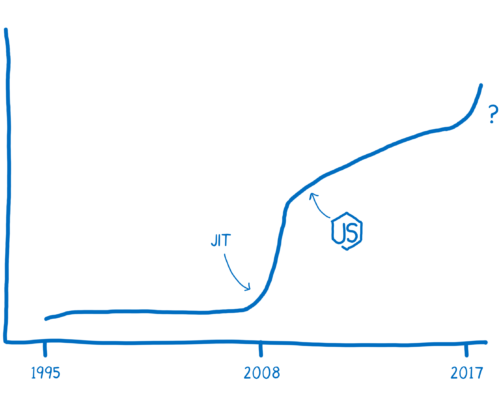
\includegraphics[width=0.7\textwidth,height=0.7\textheight]{./images/perf_history.png}
        \caption{\href{https://hacks.mozilla.org/2017/02/a-cartoon-intro-to-webassembly/}{Performance-Entwicklung im Web-Kontext}}
    \end{figure}
\end{frame}

\begin{frame}{Definition}
    \begin{figure}
        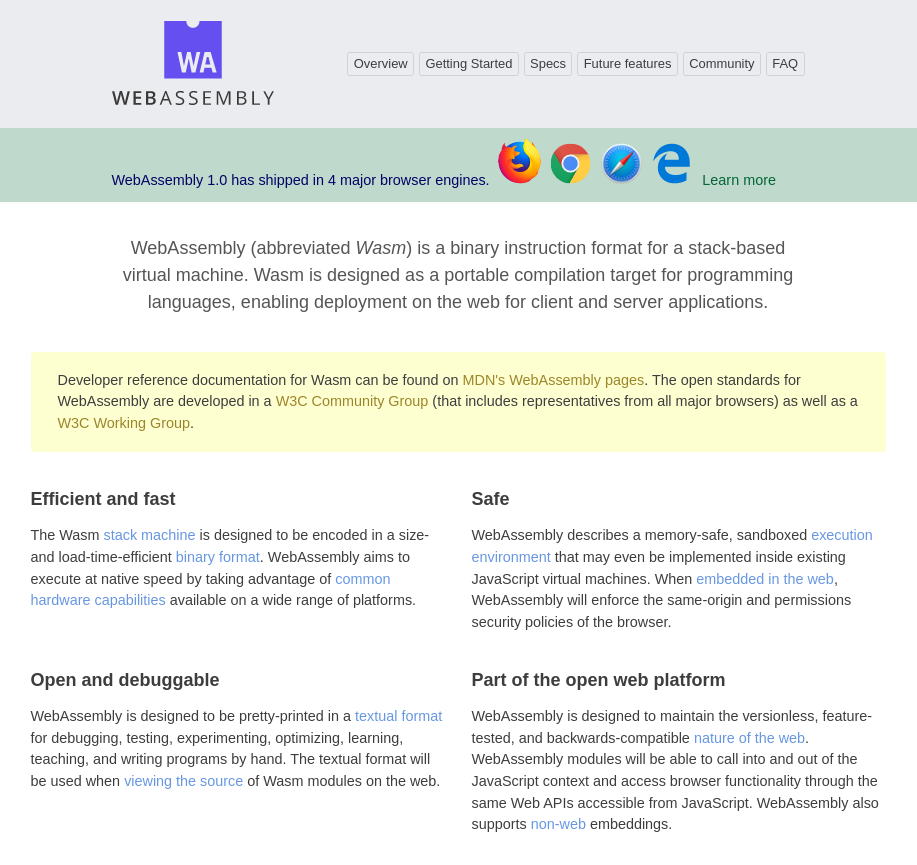
\includegraphics[scale=0.2]{./images/webassembly_org.png}
        \caption{\href{https://webassembly.org/}{Webassembly.org}}
    \end{figure}
\end{frame}

\begin{frame}{Definition}
\begin{quotation}
"WebAssembly (abbreviated Wasm) is a binary instruction format for a stack-based virtual machine. Wasm is designed as a portable compilation target for programming languages, enabling deployment on the web for client and server applications."
\end{quotation}
\end{frame}

\end{document}
